% removed leading markdown fence
\chapter{Reinforcement Learning---The Dance Between Agent and Environment}

\begin{quote}
    \itshape
    ``We learn by doing, and we learn best when the consequences of our actions are immediate and clear.''
    
    \raggedleft--- Edward Thorndike, \textit{Law of Effect}
\end{quote}

\begin{quote}
    \itshape
    ``All life is problem solving.''
    
    \raggedleft--- Karl Popper
\end{quote}

\section{Introduction: From Passive Observation to Active Intervention}

\subsection{The Philosophical Shift from Supervised to Reinforcement Learning}

In the previous chapters, we explored methods where knowledge emerges from \textit{observation}---clustering discovers latent structure, classification learns from labeled examples. But the crown jewel of machine learning is \textbf{Reinforcement Learning (RL)}, where an agent learns not by passive observation but through \textit{active intervention} in its environment.

\begin{philobox}
\textbf{The Reward Hypothesis: Teleology in Algorithms}

At the heart of RL lies the \textbf{Reward Hypothesis}:

\begin{center}
\itshape
``All goals and purposes can be thought of as the maximization \\
of the expected value of the cumulative sum of a received scalar signal (reward).''
\end{center}

This hypothesis is profoundly \textit{teleological}---it assumes that behavior is goal-directed, oriented toward a future state of affairs. Unlike the mechanistic causality of physics (past causes determine present effects), RL embodies Aristotelian \textit{final causality}: actions are chosen because of their anticipated consequences.

The reward signal is not just a number---it is the \textit{ought} that guides the \textit{is}. The agent's task is to bridge David Hume's famous is-ought gap through learning.
\end{philobox}

\subsection{Reinforcement Learning as Epistemic Process}

RL faces a unique epistemological challenge: the agent must learn about the world \textit{while simultaneously changing it}. This is the problem of \textbf{learning under intervention}:

\begin{itemize}
    \item \textbf{Supervised Learning}: $P(\text{label} \mid \text{features})$ --- passive observation
    \item \textbf{Reinforcement Learning}: $P(\text{state}' \mid \text{state}, \text{action})$ --- active intervention
\end{itemize}

The agent is both \textit{observer} and \textit{participant}, both \textit{scientist} conducting experiments and \textit{subject} of those experiments. This dual role creates fundamental tensions:

\begin{enumerate}
    \item \textbf{Exploration vs. Exploitation}: Should the agent gather more data (explore) or act on current knowledge (exploit)?
    
    \item \textbf{Credit Assignment}: Which past actions led to current rewards? (The temporal credit assignment problem)
    
    \item \textbf{Epistemic vs. Aleatoric Uncertainty}: 
    \begin{itemize}
        \item \textit{Epistemic uncertainty}: Reducible ignorance about environment dynamics
        \item \textit{Aleatoric uncertainty}: Irreducible randomness in environment transitions
    \end{itemize}
\end{enumerate}

\begin{remark}[The Two Sources of Uncertainty in RL]
Following the distinction from Disentangling Epistemic and Aleatoric Uncertainty in RL:

\textbf{Epistemic Uncertainty} arises from limited data/experience. It answers: ``How confident am I in my model of the world?'' This uncertainty \textit{should} drive exploration---we explore regions where our model is uncertain.

\textbf{Aleatoric Uncertainty} arises from inherent stochasticity. Even with infinite data, a die roll remains unpredictable. This uncertainty \textit{should not} drive exploration---gathering more data won't reduce it.

Confusing these leads to pathological behaviors: over-exploring deterministic regions (epistemic error) or under-exploring truly random regions (aleatoric error).
\end{remark}

\section{Mathematical Foundations: The Markov Decision Process}

\subsection{Formal Definition}

\begin{seanbox}{5.1}
\textbf{Markov Decision Process (MDP):}

An MDP is a tuple $\mathcal{M} = (\mathcal{S}, \mathcal{A}, P, R, \gamma)$ where:

\begin{itemize}
    \item $\mathcal{S}$: State space (where the agent can be)
    \item $\mathcal{A}$: Action space (what the agent can do)
    \item $P: \mathcal{S} \times \mathcal{A} \times \mathcal{S} \to [0,1]$: Transition probability
    \begin{equation}
        P(s' \mid s, a) = \Pr(S_{t+1} = s' \mid S_t = s, A_t = a)
    \end{equation}
    
    \item $R: \mathcal{S} \times \mathcal{A} \to \mathbb{R}$: Reward function
    \begin{equation}
        R(s, a) = \mathbb{E}[R_{t+1} \mid S_t = s, A_t = a]
    \end{equation}
    
    \item $\gamma \in [0, 1)$: Discount factor (temporal preference)
\end{itemize}

\textbf{The Markov Property:}

\begin{equation}
    P(s_{t+1} \mid s_t, a_t, s_{t-1}, a_{t-1}, \ldots, s_0, a_0) = P(s_{t+1} \mid s_t, a_t)
\end{equation}

The future depends only on the present, not the path taken to reach it.

\textbf{Policy:} A mapping from states to actions

\begin{itemize}
    \item Deterministic: $\pi: \mathcal{S} \to \mathcal{A}$
    \item Stochastic: $\pi: \mathcal{S} \times \mathcal{A} \to [0, 1]$ where $\pi(a \mid s) = \Pr(A_t = a \mid S_t = s)$
\end{itemize}

\textbf{Return:} Discounted cumulative reward

\begin{equation}
    G_t = R_{t+1} + \gamma R_{t+2} + \gamma^2 R_{t+3} + \cdots = \sum_{k=0}^{\infty} \gamma^k R_{t+k+1}
\end{equation}

\textbf{Objective:} Find optimal policy $\pi^*$ that maximizes expected return

\begin{equation}
    \pi^* = \argmax_\pi \mathbb{E}_\pi\left[ G_0 \right]
\end{equation}
\end{seanbox}

\begin{philobox}
\textbf{The Markov Property as Philosophical Assumption}

The Markov property---that the present state suffices to predict the future---is not merely a mathematical convenience. It embodies a \textit{metaphysical commitment}:

\begin{center}
\itshape
``All information relevant to future outcomes is encoded in the present state.''
\end{center}

This is a form of \textbf{informational determinism}: the state is a \textit{sufficient statistic} for decision-making. If we accept this, then optimal decisions can be made using only current information---no need to remember the entire history.

But what if the Markov property is violated? What if the environment has \textit{hidden state}---aspects not observable but causally relevant? Then we face a \textbf{Partially Observable MDP (POMDP)}, where the agent must \textit{infer} the true state from observations. This mirrors the human condition: we perceive the world through limited senses, never accessing reality directly (Kant's \textit{noumena} vs. \textit{phenomena}).

The notation $P(s' \mid s, a)$ thus represents an \textit{epistemic ideal}---a perfect model of causality. In practice, we always work with approximations, introducing irreducible epistemic uncertainty.
\end{philobox}

\subsection{Value Functions: Quantifying Goodness}

\begin{seanbox}{5.2}
\textbf{State-Value Function:}

Expected return starting from state $s$ and following policy $\pi$

\begin{equation}
    V^\pi(s) = \mathbb{E}_\pi\left[ G_t \mid S_t = s \right] = \mathbb{E}_\pi\left[ \sum_{k=0}^{\infty} \gamma^k R_{t+k+1} \mid S_t = s \right]
\end{equation}

\textbf{Action-Value Function (Q-Function):}

Expected return starting from state $s$, taking action $a$, then following $\pi$

\begin{equation}
    Q^\pi(s, a) = \mathbb{E}_\pi\left[ G_t \mid S_t = s, A_t = a \right]
\end{equation}

\textbf{Relationship:}

\begin{equation}
    V^\pi(s) = \sum_{a \in \mathcal{A}} \pi(a \mid s) Q^\pi(s, a)
\end{equation}

For deterministic policy: $V^\pi(s) = Q^\pi(s, \pi(s))$

\textbf{Bellman Equations:}

The value functions satisfy recursive relationships (the Bellman equations):

\begin{align}
    V^\pi(s) &= \sum_{a} \pi(a \mid s) \left[ R(s, a) + \gamma \sum_{s'} P(s' \mid s, a) V^\pi(s') \right] \\
    Q^\pi(s, a) &= R(s, a) + \gamma \sum_{s'} P(s' \mid s, a) \sum_{a'} \pi(a' \mid s') Q^\pi(s', a')
\end{align}

\textbf{Optimal Value Functions:}

\begin{align}
    V^*(s) &= \max_\pi V^\pi(s) = \max_a Q^*(s, a) \\
    Q^*(s, a) &= R(s, a) + \gamma \sum_{s'} P(s' \mid s, a) V^*(s')
\end{align}

\textbf{Bellman Optimality Equation:}

\begin{equation}
    V^*(s) = \max_a \left[ R(s, a) + \gamma \sum_{s'} P(s' \mid s, a) V^*(s') \right]
\end{equation}

\textbf{Optimal Policy:}

\begin{equation}
    \pi^*(s) = \argmax_a Q^*(s, a)
\end{equation}

Once we have $Q^*$, acting optimally is trivial: always choose the action with highest Q-value.
\end{seanbox}

\begin{philobox}
\textbf{The Bellman Equation as Recursive Epistemology}

Richard Bellman's equation is a mathematical miracle:

\begin{equation}
    V^\pi(s) = \mathbb{E}_\pi\left[ R_{t+1} + \gamma V^\pi(S_{t+1}) \mid S_t = s \right]
\end{equation}

It says: ``The value of where you are equals the immediate reward plus the (discounted) value of where you'll be next.''

This is \textbf{backward induction} formalized---the same principle used in game theory, dynamic programming, and rational decision-making. It embodies the idea that:

\begin{center}
\itshape
``To evaluate the present, consult the (expected) future.''
\end{center}

The notation $V^\pi(s)$ is not just a number---it's a \textit{summary of all possible futures} from state $s$. It collapses an infinite tree of possibilities into a single scalar. This is \textit{abstraction} in its purest form: forgetting details while preserving essence.

The recursive structure mirrors mathematical induction:
\begin{itemize}
    \item \textbf{Base case}: Terminal states have value 0 (or immediate reward)
    \item \textbf{Inductive step}: Value of current state defined via values of successor states
\end{itemize}

Solving the Bellman equation is thus a form of \textit{epistemic bootstrapping}---we build knowledge of values by assuming we already have it, iterating until convergence. This is the essence of \textbf{fixed-point iteration}: find $V$ such that $V = \mathcal{T}V$ (where $\mathcal{T}$ is the Bellman operator).
\end{philobox}

\subsection{Visualization: The RL Feedback Loop}

\begin{visualbox}
\textbf{The Agent-Environment Interface:}

\begin{center}
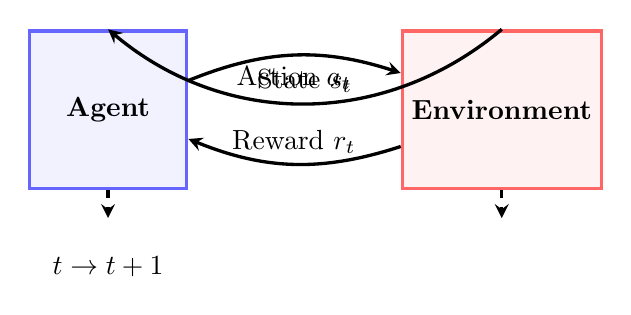
\begin{tikzpicture}[
    node distance=3cm,
    agent/.style={rectangle, draw=blue!60, fill=blue!5, very thick, minimum size=2cm},
    env/.style={rectangle, draw=red!60, fill=red!5, very thick, minimum size=2cm},
    arrow/.style={->, >=stealth, very thick}
]
    % Nodes
    \node[agent] (agent) {\textbf{Agent}};
    \node[env, right of=agent, node distance=5cm] (env) {\textbf{Environment}};
    
    % State arrow
    \draw[arrow, bend left=40] (env.north) to node[above] {State $s_t$} (agent.north);
    
    % Reward arrow
    \draw[arrow, bend left=20] (env) to node[above] {Reward $r_t$} (agent);
    
    % Action arrow
    \draw[arrow, bend left=20] (agent) to node[below] {Action $a_t$} (env);
    
    % Time advancement
    \node[below of=agent, node distance=1.5cm] (time_agent) {};
    \node[below of=env, node distance=1.5cm] (time_env) {};
    \draw[arrow, dashed] (agent) -- (time_agent);
    \draw[arrow, dashed] (env) -- (time_env);
    \node[below of=agent, node distance=2cm] {$t \to t+1$};
\end{tikzpicture}
\end{center}

\textbf{Timeline of Interaction:}

\begin{center}
\begin{tikzpicture}[scale=1.2]
    % Time axis
    \draw[->] (0,0) -- (12,0) node[right] {Time};
    
    % Time points
    \foreach \x/\t in {1/0, 3/1, 5/2, 7/3, 9/\cdots, 11/T} {
        \draw (\x,0.1) -- (\x,-0.1) node[below] {$t=\t$};
    }
    
    % States
    \foreach \x/\s in {1/s_0, 3/s_1, 5/s_2, 7/s_3, 11/s_T} {
        \node[circle, draw, fill=blue!20] at (\x, 1.5) {$\s$};
    }
    
    % Actions
    \foreach \x/\a in {2/a_0, 4/a_1, 6/a_2, 8/a_3} {
        \node[rectangle, draw, fill=green!20] at (\x, 0.75) {$\a$};
    }
    
    % Rewards
    \foreach \x/\r in {3/r_1, 5/r_2, 7/r_3, 11/r_T} {
        \node[diamond, draw, fill=red!20, aspect=2] at (\x, 2.25) {$\r$};
    }
    
    % Arrows
    \foreach \x in {1,3,5,7} {
        \draw[->] (\x,1.3) -- (\x+1,0.95);
        \draw[->] (\x+1,0.75) -- (\x+2,1.3);
        \draw[->] (\x+2,1.7) -- (\x+2,2.0);
    }
\end{tikzpicture}
\end{center}

The agent and environment engage in a temporal loop: the agent observes $s_t$, selects $a_t$, receives $r_{t+1}$ and $s_{t+1}$, then repeats. This is the fundamental rhythm of learning through interaction.
\end{visualbox}

\section{Dynamic Programming: Exact Solution Methods}

When the MDP model $(P, R)$ is \textit{known}, we can solve for optimal policies exactly using dynamic programming.

\subsection{Policy Iteration}

\begin{seanbox}{5.3}
\textbf{Policy Iteration Algorithm:}

\begin{algorithmic}[1]
\State Initialize $\pi_0$ arbitrarily
\For{$k = 0, 1, 2, \ldots$ until convergence}
    \State \textbf{Policy Evaluation:} Compute $V^{\pi_k}$ by solving
    \begin{equation}
        V^{\pi_k}(s) = \sum_a \pi_k(a \mid s) \left[ R(s,a) + \gamma \sum_{s'} P(s' \mid s, a) V^{\pi_k}(s') \right]
    \end{equation}
    (This is a system of $|\mathcal{S}|$ linear equations)
    
    \State \textbf{Policy Improvement:} Compute greedy policy
    \begin{equation}
        \pi_{k+1}(s) = \argmax_a \left[ R(s,a) + \gamma \sum_{s'} P(s' \mid s, a) V^{\pi_k}(s') \right]
    \end{equation}
\EndFor
\end{algorithmic}

\textbf{Convergence:} Policy iteration converges to $\pi^*$ in finite iterations.

\textbf{Why it works:} Policy improvement is monotonic
\begin{equation}
    V^{\pi_{k+1}}(s) \geq V^{\pi_k}(s) \quad \forall s
\end{equation}

Since there are finitely many policies and improvement is strict (unless already optimal), convergence is guaranteed.
\end{seanbox}

\subsection{Value Iteration}

\begin{seanbox}{5.4}
\textbf{Value Iteration Algorithm:}

Instead of alternating evaluation and improvement, directly iterate the Bellman optimality equation:

\begin{algorithmic}[1]
\State Initialize $V_0(s)$ arbitrarily (e.g., $V_0(s) = 0 \, \forall s$)
\For{$k = 0, 1, 2, \ldots$ until convergence}
    \For{all $s \in \mathcal{S}$}
        \State $V_{k+1}(s) = \max_a \left[ R(s,a) + \gamma \sum_{s'} P(s' \mid s, a) V_k(s') \right]$
    \EndFor
\EndFor
\State Extract policy: $\pi(s) = \argmax_a \left[ R(s,a) + \gamma \sum_{s'} P(s' \mid s, a) V(s') \right]$
\end{algorithmic}

\textbf{Convergence:} The Bellman operator is a $\gamma$-contraction, so $V_k \to V^*$ exponentially fast.

\textbf{Computational cost per iteration:} $O(|\mathcal{S}|^2 |\mathcal{A}|)$
\end{seanbox}

\begin{visualbox}
\textbf{Value Iteration Convergence (Gridworld Example):}

\begin{center}
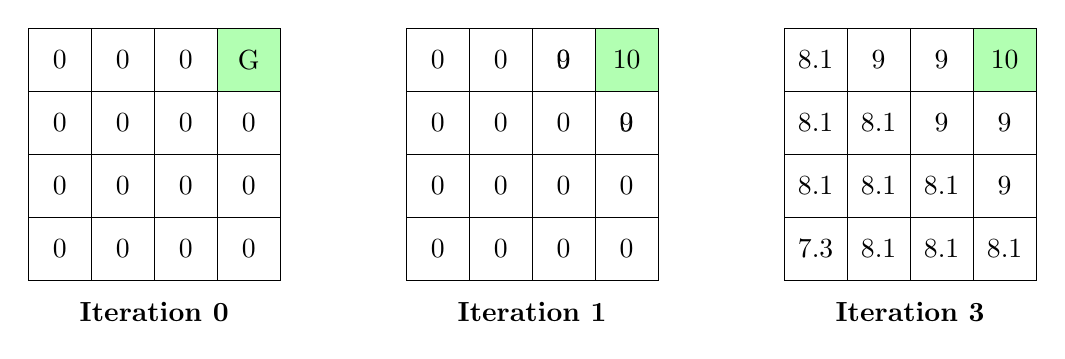
\begin{tikzpicture}[scale=0.8]
    % Initial V0 = 0
    \begin{scope}
        \node at (2, -0.5) {\textbf{Iteration 0}};
        \foreach \x in {0,1,2,3} {
            \foreach \y in {0,1,2,3} {
                \draw (\x, \y) rectangle (\x+1, \y+1);
                \node at (\x+0.5, \y+0.5) {0};
            }
        }
        % Goal state
        \draw[fill=green!30] (3,3) rectangle (4,4);
        \node at (3.5, 3.5) {G};
    \end{scope}
    
    % After iteration 1
    \begin{scope}[xshift=6cm]
        \node at (2, -0.5) {\textbf{Iteration 1}};
        \foreach \x in {0,1,2,3} {
            \foreach \y in {0,1,2,3} {
                \draw (\x, \y) rectangle (\x+1, \y+1);
                \node at (\x+0.5, \y+0.5) {0};
            }
        }
        % Goal state
        \draw[fill=green!30] (3,3) rectangle (4,4);
        \node at (3.5, 3.5) {10};
        % Adjacent to goal
        \node at (2.5, 3.5) {9};
        \node at (3.5, 2.5) {9};
    \end{scope}
    
    % After iteration 3
    \begin{scope}[xshift=12cm]
        \node at (2, -0.5) {\textbf{Iteration 3}};
        % Values propagate
        \foreach \x/\y/\v in {0/0/7.3, 1/0/8.1, 2/0/8.1, 3/0/8.1,
                              0/1/8.1, 1/1/8.1, 2/1/8.1, 3/1/9,
                              0/2/8.1, 1/2/8.1, 2/2/9, 3/2/9,
                              0/3/8.1, 1/3/9, 2/3/9} {
            \draw (\x, \y) rectangle (\x+1, \y+1);
            \node at (\x+0.5, \y+0.5) {\v};
        }
        \draw[fill=green!30] (3,3) rectangle (4,4);
        \node at (3.5, 3.5) {10};
    \end{scope}
\end{tikzpicture}
\end{center}

Values propagate from the goal state (reward source) backward through the state space. After sufficient iterations, every state knows its value (expected return to goal).
\end{visualbox}

\section{Temporal Difference Learning: Learning from Experience}

Dynamic programming requires knowing $P$ and $R$---the full MDP model. In most real-world scenarios, we don't have this luxury. We must learn from \textit{experience}---samples of $(s, a, r, s')$ transitions.

\subsection{Monte Carlo Methods}

\begin{definition}[Monte Carlo Estimation]
Estimate $V^\pi(s)$ by averaging actual returns from episodes starting in $s$:

\begin{equation}
    V^\pi(s) \approx \frac{1}{N} \sum_{i=1}^N G_i(s)
\end{equation}

where $G_i(s)$ is the return from episode $i$ starting in state $s$.
\end{definition}

\textbf{Limitation:} Requires complete episodes (episodic tasks). Cannot learn online.

\subsection{Temporal Difference (TD) Learning}

The breakthrough: learn from incomplete episodes using \textit{bootstrapping}.

\begin{seanbox}{5.5}
\textbf{TD(0) Learning:}

After observing transition $(s, a, r, s')$, update value estimate:

\begin{equation}
    V(s) \leftarrow V(s) + \alpha \left[ \underbrace{r + \gamma V(s')}_{\text{TD target}} - \underbrace{V(s)}_{\text{current estimate}} \right]
\end{equation}

The term in brackets is the \textbf{TD error}:

\begin{equation}
    \delta_t = R_{t+1} + \gamma V(S_{t+1}) - V(S_t)
\end{equation}

\textbf{Key insight:} Use the current estimate $V(s')$ as a proxy for the true future return. This is \textit{bootstrapping}---pulling yourself up by your own bootstraps.

\textbf{Comparison:}

\begin{itemize}
    \item \textbf{Monte Carlo}: $V(S_t) \leftarrow V(S_t) + \alpha [G_t - V(S_t)]$ \quad (actual return)
    \item \textbf{TD(0)}: $V(S_t) \leftarrow V(S_t) + \alpha [R_{t+1} + \gamma V(S_{t+1}) - V(S_t)]$ \quad (estimated return)
\end{itemize}

TD learns from every transition; MC learns only at episode end.
\end{seanbox}

\begin{philobox}
\textbf{Bootstrapping as Epistemic Circularity}

TD learning is philosophically remarkable: it uses the \textit{current} value estimate to improve itself. This seems circular---how can you learn truth from your own ignorance?

The answer lies in the \textit{iterative nature}: each estimate is slightly better than the last. Over time, errors cancel out and the estimates converge to truth. This is analogous to:

\begin{itemize}
    \item \textbf{Hermeneutic circle} (philosophy): Understanding the whole requires understanding the parts, and vice versa. We spiral inward toward comprehension.
    
    \item \textbf{Fixed-point iteration} (mathematics): Solve $x = f(x)$ by iterating $x_{n+1} = f(x_n)$.
    
    \item \textbf{Reflective equilibrium} (ethics): Moral principles and particular judgments adjust each other until coherence is reached.
\end{itemize}

The notation $\delta_t = r + \gamma V(s') - V(s)$ captures the \textit{surprise}---the gap between prediction and reality. Learning is driven by surprise: when outcomes match expectations ($\delta = 0$), no update occurs. This mirrors Bayesian updating: evidence that confirms beliefs has no effect.

TD learning embodies \textbf{pragmatism}: truth is what \textit{works}. We don't need the ``true'' value function---we need one that makes good decisions. The criterion is predictive success, not correspondence to reality.
\end{philobox}

\section{Q-Learning: Learning Optimal Action-Values}

\subsection{The Q-Learning Algorithm}

\begin{seanbox}{5.6}
\textbf{Q-Learning (Off-Policy TD Control):}

Learn $Q^*(s, a)$ directly without needing a model of the environment.

\textbf{Algorithm:}

\begin{algorithmic}[1]
\State Initialize $Q(s, a)$ arbitrarily (e.g., $Q(s, a) = 0 \, \forall s, a$)
\For{each episode}
    \State Initialize $s$
    \For{each step of episode}
        \State Choose $a$ from $s$ using policy derived from $Q$ (e.g., $\epsilon$-greedy)
        \State Take action $a$, observe $r, s'$
        \State $Q(s, a) \leftarrow Q(s, a) + \alpha \left[ r + \gamma \max_{a'} Q(s', a') - Q(s, a) \right]$
        \State $s \leftarrow s'$
    \EndFor
\EndFor
\end{algorithmic}

\textbf{Key property:} Off-policy---learns optimal policy while following a different (exploratory) policy.

\textbf{Update rule:}

\begin{equation}
    Q(s, a) \leftarrow Q(s, a) + \alpha \underbrace{\left[ r + \gamma \max_{a'} Q(s', a') - Q(s, a) \right]}_{\text{TD error for Q}}
\end{equation}

The $\max$ operator makes Q-learning learn the \textit{optimal} action-value function, regardless of the policy being followed.

\textbf{Convergence:} Under standard conditions (all state-action pairs visited infinitely often, learning rate decays appropriately), $Q \to Q^*$.
\end{seanbox}

\subsection{Exploration Strategies}

\begin{definition}[$\epsilon$-Greedy Policy]
With probability $\epsilon$, choose random action (explore); otherwise choose greedy action (exploit):

\begin{equation}
    a = \begin{cases}
        \text{random action} & \text{with probability } \epsilon \\
        \argmax_a Q(s, a) & \text{with probability } 1 - \epsilon
    \end{cases}
\end{equation}

Common schedule: $\epsilon_t = \epsilon_0 \cdot \text{decay}^t$ (anneal exploration over time)
\end{definition}

\begin{definition}[Softmax (Boltzmann) Exploration]
Choose actions probabilistically based on Q-values:

\begin{equation}
    \pi(a \mid s) = \frac{\exp(Q(s, a) / \tau)}{\sum_{a'} \exp(Q(s, a') / \tau)}
\end{equation}

where $\tau$ is the temperature parameter (higher $\tau$ = more random).
\end{definition}

\begin{definition}[Upper Confidence Bound (UCB)]
Choose action that maximizes:

\begin{equation}
    a^* = \argmax_a \left[ Q(s, a) + c \sqrt{\frac{\ln N(s)}{N(s, a)}} \right]
\end{equation}

where $N(s, a)$ is the number of times action $a$ was taken in state $s$. The second term is an \textit{exploration bonus}---favors rarely-tried actions.
\end{definition}

\begin{philobox}
\textbf{Exploration as Epistemic Virtue}

The exploration-exploitation dilemma is not just an algorithmic challenge---it's a fundamental tension in epistemology:

\begin{itemize}
    \item \textbf{Exploitation}: Use current knowledge to maximize reward (pragmatism)
    \item \textbf{Exploration}: Gather information to improve future decisions (epistemic responsibility)
\end{itemize}

Pure exploitation is \textit{dogmatism}---acting on beliefs without questioning them. Pure exploration is \textit{skepticism}---endlessly gathering data without committing to action.

The optimal balance depends on:
\begin{enumerate}
    \item \textbf{Time horizon}: Short-term goals favor exploitation; long-term goals favor exploration
    \item \textbf{Epistemic uncertainty}: High uncertainty demands exploration
    \item \textbf{Cost of error}: In safety-critical domains, cautious exploration is essential
\end{enumerate}

The $\epsilon$-greedy policy is philosophically naive---it treats all uncertainties equally. UCB is more sophisticated: it directs exploration toward regions of high \textit{epistemic} uncertainty (rarely-visited state-actions), ignoring aleatoric uncertainty (inherent randomness).

This mirrors the scientific method: design experiments to maximize \textit{information gain}, not to confirm existing beliefs.
\end{philobox}

\subsection{Code Implementation}

\begin{codebox}
\textbf{Q-Learning on GridWorld:}

\begin{lstlisting}
import numpy as np
import matplotlib.pyplot as plt

class GridWorld:
    def __init__(self, size=5):
        self.size = size
        self.goal = (size-1, size-1)
        self.state = (0, 0)
        
    def reset(self):
        self.state = (0, 0)
        return self._state_to_idx(self.state)
    
    def step(self, action):
        # Actions: 0=up, 1=right, 2=down, 3=left
        moves = [(-1,0), (0,1), (1,0), (0,-1)]
        dy, dx = moves[action]
        new_y, new_x = self.state[0] + dy, self.state[1] + dx
        
        # Boundary check
        if 0 <= new_y < self.size and 0 <= new_x < self.size:
            self.state = (new_y, new_x)
        
        # Reward structure
        if self.state == self.goal:
            reward = 10.0
            done = True
        else:
            reward = -0.1  # Living penalty
            done = False
            
        return self._state_to_idx(self.state), reward, done
    
    def _state_to_idx(self, state):
        return state[0] * self.size + state[1]

# Q-Learning
def q_learning(env, episodes=1000, alpha=0.1, gamma=0.95, epsilon=0.1):
    n_states = env.size ** 2
    n_actions = 4
    Q = np.zeros((n_states, n_actions))
    
    rewards_per_episode = []
    
    for episode in range(episodes):
        state = env.reset()
        total_reward = 0
        done = False
        
        while not done:
            # Epsilon-greedy action selection
            if np.random.rand() < epsilon:
                action = np.random.randint(n_actions)
            else:
                action = np.argmax(Q[state])
            
            # Take action
            next_state, reward, done = env.step(action)
            total_reward += reward
            
            # Q-learning update
            td_target = reward + gamma * np.max(Q[next_state])
            td_error = td_target - Q[state, action]
            Q[state, action] += alpha * td_error
            
            state = next_state
        
        rewards_per_episode.append(total_reward)
        
        # Decay epsilon
        epsilon = max(0.01, epsilon * 0.995)
    
    return Q, rewards_per_episode

# Run Q-learning
env = GridWorld(size=5)
Q, rewards = q_learning(env, episodes=2000)

# Visualize learning curve
plt.figure(figsize=(10, 5))
plt.subplot(1, 2, 1)
plt.plot(np.convolve(rewards, np.ones(50)/50, mode='valid'))
plt.xlabel('Episode')
plt.ylabel('Average Reward (smoothed)')
plt.title('Q-Learning Performance')
plt.grid(True)

# Visualize learned policy
plt.subplot(1, 2, 2)
policy = np.argmax(Q, axis=1).reshape(env.size, env.size)
arrows = {0: '^', 1: '>', 2: 'v', 3: '<'}
for i in range(env.size):
    for j in range(env.size):
        if (i, j) == env.goal:
            plt.text(j, env.size-1-i, 'G', ha='center', va='center', 
                    fontsize=20, color='green', weight='bold')
        else:
            action_idx = policy[i, j]
            plt.text(j, env.size-1-i, arrows[action_idx], 
                    ha='center', va='center', fontsize=16)
plt.xlim(-0.5, env.size-0.5)
plt.ylim(-0.5, env.size-0.5)
plt.grid(True)
plt.gca().set_aspect('equal')
plt.title('Learned Policy')
plt.tight_layout()
plt.show()

print(f"Final Q-values sample:\n{Q[:5]}")
\end{lstlisting}

\textbf{Output interpretation:}
\begin{itemize}
    \item Left plot shows reward improving over episodes (learning curve)
    \item Right plot shows learned policy as arrows (optimal actions)
    \item The policy should show arrows pointing toward the goal
\end{itemize}
\end{codebox}

\section{Deep Q-Networks (DQN): Function Approximation}

For large state spaces (e.g., images), tabular Q-learning is infeasible. Solution: approximate $Q(s, a)$ with a neural network.

\subsection{The DQN Architecture}

\begin{seanbox}{5.7}
\textbf{Deep Q-Network (DQN):}

\textbf{Q-Network:} Neural network $Q(s, a; \theta)$ with parameters $\theta$

\textbf{Loss function:} Mean squared Bellman error

\begin{equation}
    L(\theta) = \mathbb{E}_{(s,a,r,s') \sim \mathcal{D}} \left[ \left( \underbrace{r + \gamma \max_{a'} Q(s', a'; \theta^-)}_{\text{target}} - Q(s, a; \theta) \right)^2 \right]
\end{equation}

\textbf{Key innovations:}

\begin{enumerate}
    \item \textbf{Experience Replay}: Store transitions in replay buffer $\mathcal{D}$, sample mini-batches randomly
    \begin{itemize}
        \item Breaks correlation between consecutive samples
        \item Enables data reuse (sample efficiency)
    \end{itemize}
    
    \item \textbf{Target Network}: Use separate network $Q(s, a; \theta^-)$ for computing targets
    \begin{itemize}
        \item Parameters $\theta^-$ updated slowly (every $C$ steps): $\theta^- \leftarrow \theta$
        \item Stabilizes learning (target is stationary within window)
    \end{itemize}
\end{enumerate}

\textbf{Gradient:}

\begin{equation}
    \nabla_\theta L(\theta) = \mathbb{E} \left[ \left( r + \gamma \max_{a'} Q(s', a'; \theta^-) - Q(s, a; \theta) \right) \nabla_\theta Q(s, a; \theta) \right]
\end{equation}

\textbf{DQN Algorithm:}

\begin{algorithmic}[1]
\State Initialize Q-network $Q(s, a; \theta)$ and target network $Q(s, a; \theta^-)$ with $\theta^- = \theta$
\State Initialize replay buffer $\mathcal{D}$
\For{each episode}
    \State Initialize state $s$
    \For{each step}
        \State Select action: $a = \argmax_a Q(s, a; \theta)$ with probability $1-\epsilon$, else random
        \State Execute $a$, observe $r, s'$
        \State Store transition $(s, a, r, s')$ in $\mathcal{D}$
        \State Sample mini-batch from $\mathcal{D}$
        \State Compute targets: $y_i = r_i + \gamma \max_{a'} Q(s_i', a'; \theta^-)$
        \State Perform gradient descent on $(y_i - Q(s_i, a_i; \theta))^2$
        \State Every $C$ steps: $\theta^- \leftarrow \theta$
    \EndFor
\EndFor
\end{algorithmic}
\end{seanbox}

\begin{codebox}
\textbf{DQN with PyTorch (Simplified):}

\begin{lstlisting}
import torch
import torch.nn as nn
import torch.optim as optim
import numpy as np
from collections import deque
import random

class QNetwork(nn.Module):
    def __init__(self, state_dim, action_dim):
        super().__init__()
        self.net = nn.Sequential(
            nn.Linear(state_dim, 128),
            nn.ReLU(),
            nn.Linear(128, 128),
            nn.ReLU(),
            nn.Linear(128, action_dim)
        )
    
    def forward(self, state):
        return self.net(state)

class ReplayBuffer:
    def __init__(self, capacity=10000):
        self.buffer = deque(maxlen=capacity)
    
    def push(self, state, action, reward, next_state, done):
        self.buffer.append((state, action, reward, next_state, done))
    
    def sample(self, batch_size):
        batch = random.sample(self.buffer, batch_size)
        states, actions, rewards, next_states, dones = zip(*batch)
        return (np.array(states), np.array(actions), np.array(rewards),
                np.array(next_states), np.array(dones))
    
    def __len__(self):
        return len(self.buffer)

class DQNAgent:
    def __init__(self, state_dim, action_dim, lr=1e-3, gamma=0.99):
        self.action_dim = action_dim
        self.gamma = gamma
        
        # Q-network and target network
        self.q_net = QNetwork(state_dim, action_dim)
        self.target_net = QNetwork(state_dim, action_dim)
        self.target_net.load_state_dict(self.q_net.state_dict())
        
        self.optimizer = optim.Adam(self.q_net.parameters(), lr=lr)
        self.replay_buffer = ReplayBuffer()
        
    def select_action(self, state, epsilon=0.1):
        if random.random() < epsilon:
            return random.randint(0, self.action_dim - 1)
        else:
            with torch.no_grad():
                state_tensor = torch.FloatTensor(state).unsqueeze(0)
                q_values = self.q_net(state_tensor)
                return q_values.argmax().item()
    
    def train(self, batch_size=64):
        if len(self.replay_buffer) < batch_size:
            return
        
        # Sample batch
        states, actions, rewards, next_states, dones = \
            self.replay_buffer.sample(batch_size)
        
        # Convert to tensors
        states = torch.FloatTensor(states)
        actions = torch.LongTensor(actions)
        rewards = torch.FloatTensor(rewards)
        next_states = torch.FloatTensor(next_states)
        dones = torch.FloatTensor(dones)
        
        # Compute current Q-values
        current_q = self.q_net(states).gather(1, actions.unsqueeze(1)).squeeze()
        
        # Compute target Q-values
        with torch.no_grad():
            max_next_q = self.target_net(next_states).max(1)[0]
            target_q = rewards + (1 - dones) * self.gamma * max_next_q
        
        # Compute loss and update
        loss = nn.MSELoss()(current_q, target_q)
        self.optimizer.zero_grad()
        loss.backward()
        self.optimizer.step()
        
        return loss.item()
    
    def update_target_network(self):
        self.target_net.load_state_dict(self.q_net.state_dict())

# Training loop (pseudo-code, requires environment)
# agent = DQNAgent(state_dim=4, action_dim=2)
# for episode in range(1000):
#     state = env.reset()
#     for step in range(max_steps):
#         action = agent.select_action(state, epsilon=epsilon)
#         next_state, reward, done, _ = env.step(action)
#         agent.replay_buffer.push(state, action, reward, next_state, done)
#         loss = agent.train(batch_size=64)
#         if step % 100 == 0:
#             agent.update_target_network()
#         state = next_state
#         if done:
#             break
\end{lstlisting}
\end{codebox}

\section{Policy Gradient Methods: Learning Policies Directly}

Value-based methods (Q-learning, DQN) learn values, then derive policies. Policy gradient methods learn policies \textit{directly}.

\subsection{The Policy Gradient Theorem}

\begin{seanbox}{5.8}
\textbf{Policy Gradient Theorem:}

Parameterize policy: $\pi(a \mid s; \theta)$

\textbf{Objective:} Maximize expected return

\begin{equation}
    J(\theta) = \mathbb{E}_{\tau \sim \pi_\theta} \left[ \sum_{t=0}^T \gamma^t R_t \right]
\end{equation}

where $\tau = (s_0, a_0, r_0, s_1, a_1, r_1, \ldots)$ is a trajectory.

\textbf{Gradient:}

\begin{equation}
    \nabla_\theta J(\theta) = \mathbb{E}_{\tau \sim \pi_\theta} \left[ \sum_{t=0}^T \nabla_\theta \log \pi(a_t \mid s_t; \theta) \cdot G_t \right]
\end{equation}

where $G_t = \sum_{k=t}^T \gamma^{k-t} R_k$ is the return from time $t$.

\textbf{Intuition:} Increase probability of actions that led to high return.

\textbf{REINFORCE Algorithm:}

\begin{algorithmic}[1]
\State Initialize policy parameters $\theta$
\For{each episode}
    \State Generate trajectory $\tau$ following $\pi_\theta$
    \For{each time step $t$}
        \State Compute return: $G_t = \sum_{k=t}^T \gamma^{k-t} R_k$
        \State Update: $\theta \leftarrow \theta + \alpha \gamma^t G_t \nabla_\theta \log \pi(a_t \mid s_t; \theta)$
    \EndFor
\EndFor
\end{algorithmic}

\textbf{Variance reduction:} Subtract baseline $b(s_t)$ from return

\begin{equation}
    \nabla_\theta J(\theta) = \mathbb{E} \left[ \sum_t \nabla_\theta \log \pi(a_t \mid s_t; \theta) \cdot (G_t - b(s_t)) \right]
\end{equation}

Common choice: $b(s_t) = V(s_t)$ (value function baseline)
\end{seanbox}

\begin{philobox}
\textbf{Policy Gradients: Optimizing Intentionality}

Policy gradient methods are philosophically elegant: they directly optimize the \textit{agent's decision-making process}, not an intermediate value function.

The gradient $\nabla_\theta \log \pi(a \mid s; \theta)$ is the \textit{direction in parameter space} that increases the probability of action $a$. Weighting by $G_t$ means: ``If this action led to high return, move parameters in this direction.''

This is \textbf{credit assignment via gradient flow}: causality (which parameter changes caused reward) is encoded in the gradient.

The variance problem is epistemological: high-variance gradients mean \textit{noisy evidence}. Sometimes an action gets lucky (high $G_t$ due to randomness, not skill). Baselines reduce variance by asking: ``Was this return \textit{surprisingly good} compared to expectation?''

The notation $\nabla_\theta \log \pi$ is the \textbf{score function}---a likelihood-ratio trick that enables learning from samples without knowing the environment dynamics. This is REINFORCE's genius: learn from experience alone, no model needed.
\end{philobox}

\subsection{Actor-Critic Methods}

Combine policy gradients (actor) with value functions (critic).

\begin{seanbox}{5.9}
\textbf{Advantage Actor-Critic (A2C):}

\textbf{Two networks:}
\begin{itemize}
    \item \textbf{Actor}: Policy $\pi(a \mid s; \theta)$
    \item \textbf{Critic}: Value function $V(s; w)$
\end{itemize}

\textbf{Advantage function:}

\begin{equation}
    A(s, a) = Q(s, a) - V(s) \approx r + \gamma V(s') - V(s)
\end{equation}

(TD error is an unbiased estimate of advantage)

\textbf{Actor update:} Policy gradient with advantage as weight

\begin{equation}
    \theta \leftarrow \theta + \alpha_\theta \nabla_\theta \log \pi(a \mid s; \theta) \cdot A(s, a)
\end{equation}

\textbf{Critic update:} TD learning

\begin{equation}
    w \leftarrow w + \alpha_w (r + \gamma V(s'; w) - V(s; w)) \nabla_w V(s; w)
\end{equation}

\textbf{Advantage:} Lower variance than REINFORCE (uses bootstrapping)
\end{seanbox}

\begin{codebox}
\textbf{Simple A2C Implementation:}

\begin{lstlisting}
import torch
import torch.nn as nn
import torch.optim as optim
import torch.nn.functional as F

class ActorCritic(nn.Module):
    def __init__(self, state_dim, action_dim):
        super().__init__()
        # Shared layers
        self.fc1 = nn.Linear(state_dim, 128)
        
        # Actor head
        self.actor = nn.Linear(128, action_dim)
        
        # Critic head
        self.critic = nn.Linear(128, 1)
    
    def forward(self, state):
        x = F.relu(self.fc1(state))
        
        # Policy distribution
        action_probs = F.softmax(self.actor(x), dim=-1)
        
        # State value
        state_value = self.critic(x)
        
        return action_probs, state_value

class A2CAgent:
    def __init__(self, state_dim, action_dim, lr=1e-3, gamma=0.99):
        self.gamma = gamma
        self.model = ActorCritic(state_dim, action_dim)
        self.optimizer = optim.Adam(self.model.parameters(), lr=lr)
    
    def select_action(self, state):
        state_tensor = torch.FloatTensor(state).unsqueeze(0)
        action_probs, state_value = self.model(state_tensor)
        
        # Sample action from distribution
        dist = torch.distributions.Categorical(action_probs)
        action = dist.sample()
        
        return action.item(), dist.log_prob(action), state_value
    
    def train(self, log_probs, values, rewards, next_value):
        returns = []
        R = next_value
        
        # Compute returns (backward from terminal state)
        for r in reversed(rewards):
            R = r + self.gamma * R
            returns.insert(0, R)
        
        returns = torch.tensor(returns)
        log_probs = torch.cat(log_probs)
        values = torch.cat(values)
        
        # Compute advantages
        advantages = returns - values.detach()
        
        # Actor loss (policy gradient)
        actor_loss = -(log_probs * advantages).mean()
        
        # Critic loss (value function error)
        critic_loss = F.mse_loss(values, returns)
        
        # Total loss
        loss = actor_loss + 0.5 * critic_loss
        
        # Update
        self.optimizer.zero_grad()
        loss.backward()
        self.optimizer.step()
        
        return loss.item()

# Usage (pseudo-code)
# agent = A2CAgent(state_dim=4, action_dim=2)
# for episode in range(1000):
#     state = env.reset()
#     log_probs, values, rewards = [], [], []
#     
#     for step in range(max_steps):
#         action, log_prob, value = agent.select_action(state)
#         next_state, reward, done, _ = env.step(action)
#         
#         log_probs.append(log_prob)
#         values.append(value)
#         rewards.append(reward)
#         
#         state = next_state
#         if done:
#             break
#     
#     next_value = 0 if done else agent.model(torch.FloatTensor(state))[1].item()
#     loss = agent.train(log_probs, values, rewards, next_value)
\end{lstlisting}
\end{codebox}

\section{Advanced Topics}

\subsection{Proximal Policy Optimization (PPO)}

PPO is the current gold standard for policy gradient methods, used in OpenAI's GPT-4 RLHF training.

\begin{seanbox}{5.10}
\textbf{PPO Clipped Objective:}

Problem with vanilla policy gradients: large policy updates can be catastrophic.

Solution: Constrain updates to stay near current policy.

\textbf{Objective:}

\begin{equation}
    L^{\text{CLIP}}(\theta) = \mathbb{E} \left[ \min \left( \frac{\pi_\theta(a \mid s)}{\pi_{\theta_{\text{old}}}(a \mid s)} A(s, a), \, \text{clip}\left(\frac{\pi_\theta(a \mid s)}{\pi_{\theta_{\text{old}}}(a \mid s)}, 1-\epsilon, 1+\epsilon\right) A(s, a) \right) \right]
\end{equation}

The probability ratio $r(\theta) = \frac{\pi_\theta(a \mid s)}{\pi_{\theta_{\text{old}}}(a \mid s)}$ measures policy change.

Clipping to $[1-\epsilon, 1+\epsilon]$ (typically $\epsilon = 0.2$) prevents large updates.

\textbf{Advantage over TRPO}: Simpler to implement (no need for KL constraint optimization)
\end{seanbox}

\subsection{Multi-Agent Reinforcement Learning}

When multiple agents interact, the environment becomes non-stationary from each agent's perspective (other agents' policies are changing).

\begin{definition}[Markov Game]
Extension of MDP to multiple agents:

\begin{itemize}
    \item Each agent $i$ has policy $\pi_i$
    \item Transition: $P(s' \mid s, a_1, \ldots, a_n)$
    \item Each agent receives own reward: $R_i(s, a_1, \ldots, a_n)$
\end{itemize}

Solution concepts:
\begin{itemize}
    \item \textbf{Nash equilibrium}: No agent can improve by unilaterally changing policy
    \item \textbf{Cooperative}: All agents share common reward (team)
    \item \textbf{Competitive}: Zero-sum rewards (adversarial)
\end{itemize}
\end{definition}

\section{Epistemic and Aleatoric Uncertainty in RL}

\subsection{Formalizing Uncertainty}

\begin{definition}[Types of Uncertainty in RL]

\textbf{Epistemic Uncertainty} (Knowledge Uncertainty):
\begin{itemize}
    \item Uncertainty about environment dynamics: $P(s' \mid s, a)$
    \item Uncertainty about reward function: $R(s, a)$
    \item Reducible through more experience/data
    \item \textit{Should} drive exploration
\end{itemize}

\textbf{Aleatoric Uncertainty} (Inherent Randomness):
\begin{itemize}
    \item Stochasticity in transition dynamics (inherent)
    \item Stochasticity in reward (inherent)
    \item Irreducible (even with infinite data)
    \item \textit{Should not} drive exploration
\end{itemize}

\textbf{Mathematical distinction:}

\begin{align}
    \text{Epistemic:} \quad & \text{Var}[\mathbb{E}[R \mid \text{model parameters}]] \\
    \text{Aleatoric:} \quad & \mathbb{E}[\text{Var}[R \mid \text{model parameters}]]
\end{align}
\end{definition}

\begin{remark}[Importance for Safe RL]
In safety-critical applications (autonomous driving, medical treatment), distinguishing these uncertainties is crucial:

\begin{itemize}
    \item \textbf{Epistemic uncertainty}: ``I don't know what will happen'' $\to$ Be cautious, gather data
    \item \textbf{Aleatoric uncertainty}: ``This is inherently risky'' $\to$ Consider risk tolerance
\end{itemize}

Confusing them leads to:
\begin{itemize}
    \item Over-exploration of inherently random regions (wasting time)
    \item Under-exploration of deterministic but unknown regions (missing opportunities)
\end{itemize}
\end{remark}

\begin{visualbox}
\textbf{Uncertainty Decomposition:}

\begin{center}
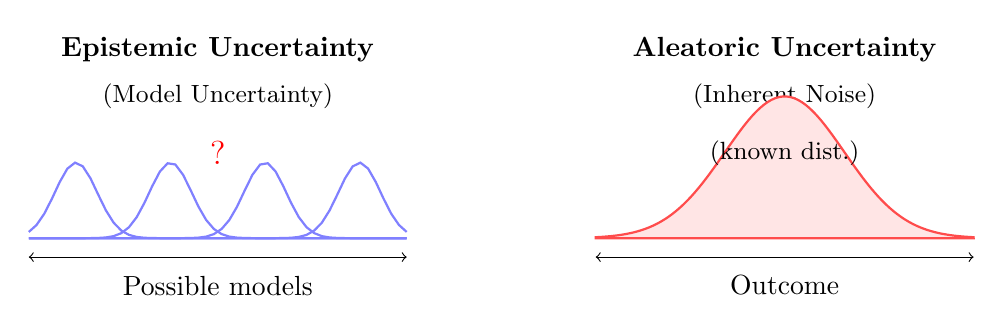
\begin{tikzpicture}[scale=1.2]
    % Epistemic uncertainty (wide distribution of means)
    \begin{scope}
        \node at (2, 3) {\textbf{Epistemic Uncertainty}};
        \node at (2, 2.5) {\small (Model Uncertainty)};
        
        % Multiple Gaussians with different means
        \foreach \mu in {0.5, 1.5, 2.5, 3.5} {
            \draw[blue!50, thick, domain=0:4, samples=50] 
                plot (\x, {0.8*exp(-(\x-\mu)^2/0.1) + 1});
        }
        
        \draw[<->] (0, 0.8) -- (4, 0.8);
        \node at (2, 0.5) {Possible models};
        \node[red, font=\large] at (2, 1.9) {?};
    \end{scope}
    
    % Aleatoric uncertainty (single distribution, inherent noise)
    \begin{scope}[xshift=6cm]
        \node at (2, 3) {\textbf{Aleatoric Uncertainty}};
        \node at (2, 2.5) {\small (Inherent Noise)};
        
        % Single Gaussian with wide variance
        \draw[red!70, thick, domain=0:4, samples=100, fill=red!10] 
            plot (\x, {1.5*exp(-(\x-2)^2/0.8) + 1}) -- (4,1) -- (0,1) -- cycle;
        
    \draw[<->] (0, 0.8) -- (4, 0.8);
    \node at (2, 0.5) {Outcome};
    % use text-checkmark to avoid glyph issues in some fonts
    \node[blue, font=\large] at (2, 2.2) {\text{\checkmark}};
    \node at (2, 1.9) {\small (known dist.)};
    \end{scope}
\end{tikzpicture}
\end{center}

\textbf{Left}: Epistemic uncertainty---we don't know which model is correct (multiple hypotheses).

\textbf{Right}: Aleatoric uncertainty---we know the distribution, but outcomes are inherently random.
\end{visualbox}

\section{Practical Considerations and Challenges}

\subsection{Sample Efficiency}

\begin{remark}[The Sample Efficiency Problem]
RL is notoriously sample-inefficient:

\begin{itemize}
    \item AlphaGo: Millions of self-play games
    \item Atari DQN: 200 million frames (approximately 924 hours of gameplay)
    \item Humans: Learn much faster from fewer examples
\end{itemize}

\textbf{Causes:}
\begin{enumerate}
    \item Temporal credit assignment (which action caused reward?)
    \item Exploration inefficiency (random exploration wastes samples)
    \item Bootstrap error propagation (errors compound through $V(s')$ estimates)
\end{enumerate}

\textbf{Solutions:}
\begin{itemize}
    \item Model-based RL (learn environment model, plan in model)
    \item Offline RL (learn from pre-collected data)
    \item Curriculum learning (start easy, increase difficulty)
    \item Meta-learning (learn to learn faster)
\end{itemize}
\end{remark}

\subsection{Reward Engineering}

\begin{philosophical}
\textbf{The Reward Specification Problem}

Designing reward functions is deceptively difficult.
\end{philosophical}
